\documentclass[12pt]{article}
\usepackage{geometry}
\usepackage{graphicx}
\usepackage{amsmath}
\usepackage{fancyhdr}
\usepackage{hyperref}

\geometry{margin=1in}

\title{Aircraft Design 1 - Fall 2024 \\ Assignment 1}
\author{Smythe Cy Goforth Jr, Matthew Burnett \\ Group 6 \\ Instance: [first delivery]}
\date{Hours spent on assignment: [35]}

\begin{document}
	
	\maketitle
	
	\section*{Aircraft Type: UAV}
	\textbf{Aircraft Number: Glider UAV Project}
	
	\begin{table}[h!]
		\centering
		\begin{tabular}{|l|c|c|}
			\hline
			Reference Type & Value & Unit \\
			\hline
			Payload & 2 & kg \\
			Range & 100 & km \\
			Altitude & 121.92 & m \\
			Cruise Speed & 10 & m/s \\
			Ceiling & 1219.2 & m \\
			Endurance & 3 & Hours \\
			Max Speed & 15 & m/s \\
			\hline
		\end{tabular}
		\caption{Basic Aircraft Specifications}
	\end{table}
	
	\newpage
	
	\tableofcontents
	
	\newpage
	
	\section{Introduction}
	The following report consists of 5 chapters, each guiding the reader through the aircraft design process. This first chapter will provide a definite mission for the aircraft and will analyze its design requirements. The second chapter will analyze reference aircraft similar in specifications to those required by the design mission, as well as include an appendix with the relevant reference material. Chapter 3 discusses the concept generation for the aircraft design and details the process of selection between the three concepts we created, and how the selected concept best meets the mission requirements. Chapter 4 will show the complete fuselage layout for the aircraft. Chapter 5 will contain technical drawings of the concept aircraft design.
	
	\section{Mission Definition and Analysis of Requirements}
	In the introduction, the basic requirements for a Low Altitude High Endurance UAV (LAHE UAV) were given. This chapter will explore FAA requirements for low-altitude UAV systems, payload specifications, and necessary design considerations.
	
	\subsection{The Mission}
	The mission for the LAHE UAV is centered around observation. The aircraft will be launched by a single operator in a remote environment, climbing to a cruise altitude of 400 meters and maintaining a cruise speed of 10 m/s. Once the cruise altitude is reached, the aircraft will enter the observation phase, utilizing a microphone sensor package to survey wildfires. The mission continues until endurance is exhausted, followed by a return to the operator, and a controlled descent and landing.
	
	\begin{figure}[h!]
		\centering
		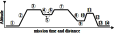
\includegraphics[width=4.5 in]{Media/MissonPlan.png} % Placeholder for technical drawings
		\caption{Technical drawings: top, side, and front views of the fuselage}
	\end{figure}
		

	\begin{enumerate}
		\item \textbf{Start Motor/s and Takeoff}: The LAHE UAV will be launched via a catapult system using an internal lithium-ion battery to power its electric motor, allowing for rapid deployment in remote environments.
		
		\item \textbf{Climb to Cruise Altitude}: The UAV will climb to 400 feet at a low angle of attack to avoid stalling due to the glider airfoil design.
		
		\item \textbf{Cruise to Survey Area}: Upon reaching cruise speed and altitude, the UAV will travel to the survey area.
		
		\item \textbf{Descend to Survey Area}: The UAV will begin its descent to the survey area while carefully managing its angle of attack to prevent stalling.
		
		\item \textbf{Loiter at Survey Area}: Once at the desired altitude, the UAV will alternate between powered flight and gliding while deploying its microphone sensor to gather data.
		
		\item \textbf{Ascend Back to Cruise Altitude}: After completing the loiter phase, the UAV will ascend back to its cruise altitude for the return trip.
		
		\item \textbf{Cruise Back to Landing Zone}: The UAV will travel back to the designated landing area, maintaining its cruise speed and altitude.
		
		\item \textbf{Descend to Landing Zone}: The UAV will descend steadily with a minimal angle of attack to prepare for landing.
		
		\item \textbf{Attempt Landing}: The UAV will attempt a soft landing by reducing its power and using a gliding approach.
		
		\item \textbf{Abort Landing if Necessary}: If conditions are not suitable, the UAV will abort its landing attempt and return to loiter over the landing zone.
		
		\item \textbf{Loiter Over Landing Zone}: The UAV will loiter and circle over the landing area, waiting for optimal landing conditions.
		
		\item \textbf{Final Descent for Landing}: After loitering, the UAV will perform a final descent with precision control.
		
		\item \textbf{Landing}: The UAV will land with fixed gear.
		
		\item \textbf{Power Off and Recover Equipment}: After landing, the UAV will power down, and the sensor equipment is recovered.
	\end{enumerate}

	\subsection{Requirement Analysis}
	\subsubsection{Payload Analysis}
	The UAV's payload consists of a microphone listening package. This microphone must be exposed outside the fuselage, increasing drag and requiring a longer wingspan. The fuselage must also include an access panel for data recovery.
	
	\subsubsection{Propulsion Analysis}
	With a proposed cruise speed of 10 m/s and a payload of 2 kg, the propulsion will be provided by a brushless electric motor. A balance between motor weight and torque output is necessary.
	
	\subsubsection{Certification Analysis}
	According to FAA regulations, the UAV must weigh under 55 pounds, fly within visual line of sight (within 3 miles), and under 400 feet of altitude, among other requirements \cite{faa_2023}.
	
	\subsubsection{Range, Takeoff, and Landing Distance}
	The UAV must cover a range of 100 km. Its endurance will be extended through efficient gliding, with minimal battery power used for propulsion.
	
	\subsubsection{Additional Requirements}
	Other requirements include minimizing power consumption, maximizing endurance, and maintaining FAA certification.
	
	\subsection{Driving Requirements}
	The critical requirements for the UAV design include range, endurance, and payload capacity, all of which influence the motor choice.
	
	\section{Reference Aircraft Data Collection}
	A range of reference aircraft were studied for inspiration and comparison. These references will provide insight into design challenges and solutions. The full reference list is included in Appendix A.
	
	\section{Concept Generation and Selection}
	\subsection{Concept Generation}
	Three design concepts were considered:
	
	\begin{itemize}
		\item Mono-pusher with inverted V-tail
		\item Dual pusher with V-tail
		\item Dual puller with cross-tail
	\end{itemize}
	
	Each concept was designed with a similar internal fuselage layout, while varying in motor and tail configurations. 'Inside-Out' sizing of the fuselage was performed after the concept selection stage.
	
	\newpage
	
	\subsubsection{Mono-pusher with Inverted V-tail}
	\begin{figure}[h!]
		\centering
		\includegraphics[width=6.5 in]{Media/MonoPusherFig.png} % Placeholder for technical drawings
		\caption{(a) The Bayraktar TB2 UAV, designed for medium altitude-long endurance surveillance and payload deployment missions \cite{}. (b) A preliminary of design of a mono pusher inverted V-tail configuration.}
	\end{figure}
	Inspired by the Bayraktar TB2, this design features a single rear-facing motor and inverted V-tail.
	
	\textbf{Pros:}
	\begin{itemize}
		\item \textbf{Higher endurance}: Preliminary calculations suggest one engine is sufficient \ref{}. Eliminating the redundant hardware of a second engine saves on weight and by extension increases fuel economy. The endurance is further aided by the reduction in drag experienced by V-tail systems. By eliminating one of the three control surfaces on a conventional configuration the drag is inevitably reduced. 
		\item \textbf{Improved structural rigidity}: The twin boom configuration considerably increases the torsional and bending rigidity of the tail section.
	\end{itemize}
	
	\textbf{Cons:}
	\begin{itemize}
		\item \textbf{Less control authority}: The reduction in control surface area reduces control authority. They are also very prone to adverse roll \cite{}.
		\item \textbf{Inefficient Yaw and Pitch}: The angled nature reduces the authority in these axes \cite{}.
	\end{itemize}
	
	To summarize, this design offers promising structural and flight efficiency characteristics but suffers in its flight control characteristics.
	
	\newpage
	
	\subsubsection{Dual Pusher with V-tail}
	\begin{figure}[h!]
		\centering
		\includegraphics[width=6.5 in]{Media/TwinPusherFig.png} % Placeholder for technical drawings
		\caption{(a) The Bayraktar TB2 UAV, designed for medium altitude-long endurance surveillance and payload deployment missions \cite{}. (b) A preliminary of design of a mono-pusher inverted V-tail configuration.}
	\end{figure}
	Inspired by the Piaggio P.180 Avanti, this concept uses twin rear-facing motors and a V-tail. No
	
	\textbf{Pros:}
	\begin{itemize}
		\item \textbf{Increased thrust}: Added thrust would enable heavier payloads and significantly reduce take-off lengths required.
		\item \textbf{Redundancy}: Having two motors would decrease the likely-hood of total engine loss.
	\end{itemize}
	
	\textbf{Cons:}
	\begin{itemize}
		\item \textbf{Reduced endurance}: The increased weight and power draw of running two motors would likely reduce the maximum endurance of the UAV.
		\item \textbf{Turbulence on control surfaces}: The pusher configuration would blow high velocity, turbulent air directly on the control surfaces. This turbulent flow could lead to reduced control authority depending on the exact aerodynamics of the aircraft.
	\end{itemize}
	
	To summarize, this design offers the potential of heavier payloads and reduced take-off runs. It also boasts more redundancy than the mono-prop design. This design however, would likely have a decreased maximum endurance and flight performance.
	
	\newpage
	
	\subsubsection{Dual Puller with Cross-tail}
	\begin{figure}[h!]
		\centering
		\includegraphics[width=6.5 in]{Media/TwinPullerFig.png} % Placeholder for technical drawings
		\caption{(a) The Bayraktar Akıncı UAV, designed for long endurance and heavy payload missions \cite{}. (b) A preliminary design of a dual puller cross-tail configuration.}
	\end{figure}
	Inspired by the Bayraktar Akıncı, this design incorporates twin forward-facing motors and a cross-tail configuration.
	
	\textbf{Pros:}
	\begin{itemize}
		\item \textbf{Higher propeller efficiency}: With forward-facing motors, the propellers operate in undisturbed air, which maximizes efficiency. 
		\item \textbf{Tail out of turbulent airflow}: The cross-tail configuration positions the control surfaces away from the turbulent air generated by the propellers, increasing control authority and efficiency. 
	\end{itemize}
	
	\textbf{Cons:}
	\begin{itemize}
		\item \textbf{Increased weight and drag}: The additional weight and drag from two engines may lead to a reduction in overall endurance.
		\item \textbf{Third tail surface increases drag}: Introducing a third control surface, increases drag compared to the V-tail configuration which could negatively affect endurance.
	\end{itemize}
	
	To summarize, this dual puller configuration offers improved propulsion efficiency and better control surface performance but may suffer from increased drag and weight, which could limit its endurance and efficiency.
	
		

	
	\subsection{Concept Selection}
	The \textbf{mono-pusher inverted V-tail} was selected. The increase endurance and structural rigidity far outweighed the challenge posed by reduced control authority and inefficient yaw and pitch. Being a UAV the standards for safety are considerably lower, so it is acceptable within the regulatory frame-work to posses only an single engine and lack control authority in some cases. The structural rigidity is crucial as this UAV needs to be able to land in undeveloped strips due to its mission objectives. Being for observation, optimizing for endurance while keeping a certain minimum payload was the primary focus. 
	
	The mono-pusher design boast the best performance in the categories being optimized for while also not posing severe challenges.
	
	\section{Preliminary Fuselage Design}
	
	\newpage
	
	\appendix
	\section{Appendix A: Reference Aircraft Data}
	
	% Include your reference data here
	
	\newpage
	
	\begin{thebibliography}{9}
		\bibitem{faa_2023}
		FAA, "14 CFR Part 48," \url{https://www.faa.gov/air_traffic/publications/atpubs/aim_html/chap11_section_2.html}, 2023.
	\end{thebibliography}
	
\end{document}
